\documentclass[licencjacka]{pracamgr}
\usepackage{polski}
\usepackage[utf8]{inputenc}
\usepackage[table]{xcolor}
\usepackage{array}
\usepackage{amssymb}
\usepackage{amsmath}
\usepackage{amsthm}
\usepackage[pdftex]{graphicx}
\usepackage{underscore}
\usepackage{hyperref}
\usepackage{caption}
\usepackage{xcolor}
\usepackage{color}
\usepackage{listings}
\hypersetup{%
    pdfborder = {0 0 0}
}
\setcounter{secnumdepth}{3}
\setcounter{tocdepth}{3}
\lstset{ %
  language=R,                     % the language of the code
  basicstyle=\footnotesize,       % the size of the fonts that are used for the code
  numbers=left,                   % where to put the line-numbers
  numberstyle=\tiny\color{gray},  % the style that is used for the line-numbers
  stepnumber=1,                   % the step between two line-numbers. If it's 1, each line
                                  % will be numbered
  numbersep=5pt,                  % how far the line-numbers are from the code
  backgroundcolor=\color{white},  % choose the background color. You must add \usepackage{color}
  showspaces=false,               % show spaces adding particular underscores
  showstringspaces=false,         % underline spaces within strings
  showtabs=false,                 % show tabs within strings adding particular underscores
  frame=single,                   % adds a frame around the code
  rulecolor=\color{black},        % if not set, the frame-color may be changed on line-breaks within not-black text (e.g. commens (green here))
  tabsize=2,                      % sets default tabsize to 2 spaces
  captionpos=b,                   % sets the caption-position to bottom
  breaklines=true,                % sets automatic line breaking
  breakatwhitespace=false,        % sets if automatic breaks should only happen at whitespace
  title=\lstname,                 % show the filename of files included with \lstinputlisting;
                                  % also try caption instead of title
  keywordstyle=\color{blue},      % keyword style
  commentstyle=\color{dkgreen},   % comment style
  stringstyle=\color{mauve},      % string literal style
  escapeinside={\%*}{*)},         % if you want to add a comment within your code
  morekeywords={*,...}            % if you want to add more keywords to the set
} 

\author{ Adam Markiewicz, Tomasz Grabowski, Albert Rozmus, Krzysztof Rutkowski, Wiktor Zuba}

\nralbumu{334774, 305145,  248353, 319379, 320501}

\title{Sugerowanie wyboru ścieżki kształcenia zintegrowane z USOS}
\tytulang{Recomendation of educational path integrated with USOS}
\kierunek{Informatyka}
\opiekun{dra Roberta Dąbrowskiego\\
Pion Zastępcy Kanclerza ds. Informatycznych}
\date{??? 2015}
\dziedzina{
11.0 Matematyka, Informatyka:\\
11.3 Informatyka\\
}
\klasyfikacja{
Information systems\\
Information systems applications\\
Decision support systems\\
Data analytics
}
%\TODO dodać litery/numery wierzchołków w klasyfikacji
\keywords{Rekomendacje \\ Predykcje \\ Wnioskowanie \\ Analiza danych}
%\newtheorem{defi}{Definicja}[section]
\graphicspath{ {./img/} }
\begin{document}
\maketitle
\begin{abstract} ~\\ \indent
Praca poświęcona jest systemowi Hermes, który ma na celu rekomendację przedmiotów dla studentów. Znajduje się w niej opis funkcjonalności, architektury, implementacji, zastosowanych algorytmów oraz organizacji pracy nad projektem.
\end{abstract}
\tableofcontents
\chapter{Wstęp}


 \section{Opis Projektu}


~\\ \indent Głównym celem projektu Hermes było stworzenie serwisu internetowego 
wspierającego studentów w procesie zoptymalizowania wyboru przedmiotów.
Serwis ma za zadanie 
umożliwić studentom lepsze planowanie ścieżki studiów i kariery zawodowej
poprzez proponowanie przedmiotów, które mogą pasować do ich upodobań i predyspozycji. 

Dodatkowym spełnionym wymaganiem projektu jest oferowanie usług przewidywania dla konkretnych studentów ocen z przedmiotów, których jescze nie ukończyli lub bądź nie podjęli.

Serwis oferuje również wsparcie dla uniwersytetu w postaci
przewidywania ilości studentów którzy zapiszą się na konkretny przedmiot. \\
\indent W celu obliczania predykcji system wykorzystywać będzie uczenie maszynowe na statystykach wszystkich studentów Uniwersytetu, a także ewentualnie wybrane przedmioty i uzyskane oceny przez studenta proszącego o propozycję. \\ \\
\indent Projekt został zrealizowany na zlecenie działu sieci komputerowych Uniwersytetu Warszawskiego.
\newpage
\section{od Autorów}

~\\ \indent Wybraliśmy ten projekt, ponieważ sami jesteśmy studentami i jesteśmy świadomi trudności związanych z wyborem przedmiotów. Oferta programowa Uniwersytetu Warszawskiego jest ogromna. W chwili pisania tej pracy po wyszukaniu w systemie usos zwróconych jest ponad 20000 przedmiotów! Dodatkowo opisy często są niejasne, szczątkowe, bądź brakuje syllabusu. Czasem tematyka przedmiotu obieralnego jest na tyle odmienna od dotychczasowego materiału poznanego przez studenta, że może on nie być świadomym, czy dany materiał odpowiada jego predyspozycjom i preferencjom.
\\ \indent Pragniemy zaadresować te problemy za pomocą systemu Hermes. Pisząc go, przyświecała nam idea stworzenia drogowskazu dla studentów, którzy nie są pewni, w jakim kierunku powinni się specjalizować. Wierzymy, iż system dzięki udanym sugestiom zwiększy liczbę studentów, którzy będą naprawdę zainteresowani tematyką przedmiotu, a zmniejszy liczbę studentów zapisanych na przedmioty zupełnie niedopasowane do ich predyspozycji, co często kończy się słabą oceną bądź nawet brakiem zaliczenia. Dzięki temu skorzystają na tym studenci, którzy z większym prawdopodobieństwem zapiszą się na pasujące do ich osiągnięć i predyspozycji przedmioty, z których zdobędą możliwie wiele interesującej ich wiedzy. Zmniejszy się również dla nich ryzyko zapisania się na przedmiot, który w ogóle nie pasuje do ich zainteresowań. Zyska również Uniwersytet, którego studenci będą bardziej zadowoleni z oferty programowej, wzrośnie jakość wiedzy absolwentów oraz lepiej zostanie wykorzystany potencjał studentów. Pomoże to uczelnii być lepiej postrzeganą, bardziej pożądaną przez przyszłych studentów a także zwiększć jej prestiż.
\\ 
\begin{flushright}
Tomasz Grabowski \\
Adam Markiewicz \\
Albert Rozmus \\
Krzysztof Rutkowski \\
Wiktor Zuba 
\end{flushright}

\chapter{Funkcjonalności}
~\\ \indent
Przy wejciu na stronę systemu użytkownik otrzymuje stronę startową która jest jednocześnie interfejsem. \\ \par
~\\
\begin{minipage}{\linewidth}
	 \centering
           
\includegraphics[scale=0.5]{home.jpg}
	\text{Ekran startowy strony}
\end{minipage} \\ \\ \\

 Poniższe podrozdziały opisują funkcjonalności zależne od wybranej opcji.

\section{Funkcjonalności dla Studentów}

\subsection{Użytkownik anonimowy}
~\\ \indent
W tym podrozdziale znajduje się opis funkcjonalności dostępnych dla użytkownika anonimowego - w domyśle studenta.
~\\


W przypadku wyboru zakładki "wprowadź oceny" student uzyskuje możliwość wprowadzenia danych dotyczacych statystyki jego zaliczeń przedmiotów w celu uzyskania nastepujących predykcji: predykcja oceny z przedmiotu, rekomendacja seminarium oraz rekomendacja przedmiotów na podstawie osiągnięć bądź rekomendacja przedmiotów dla wybranego seminarium. Intefejs ten umozliwia dodawanie dowolnej liczby przedmiotów za pomocą przycisku "plus". Dodatkowo przy wpisywaniu nazwy przedmiotu pojawia się podpowiedź sugerująca istniejące nazwy przedmiotów z bazy pasujące do wpisanego wzorca.   \par
~\\
\begin{minipage}{\linewidth}
	\centering
           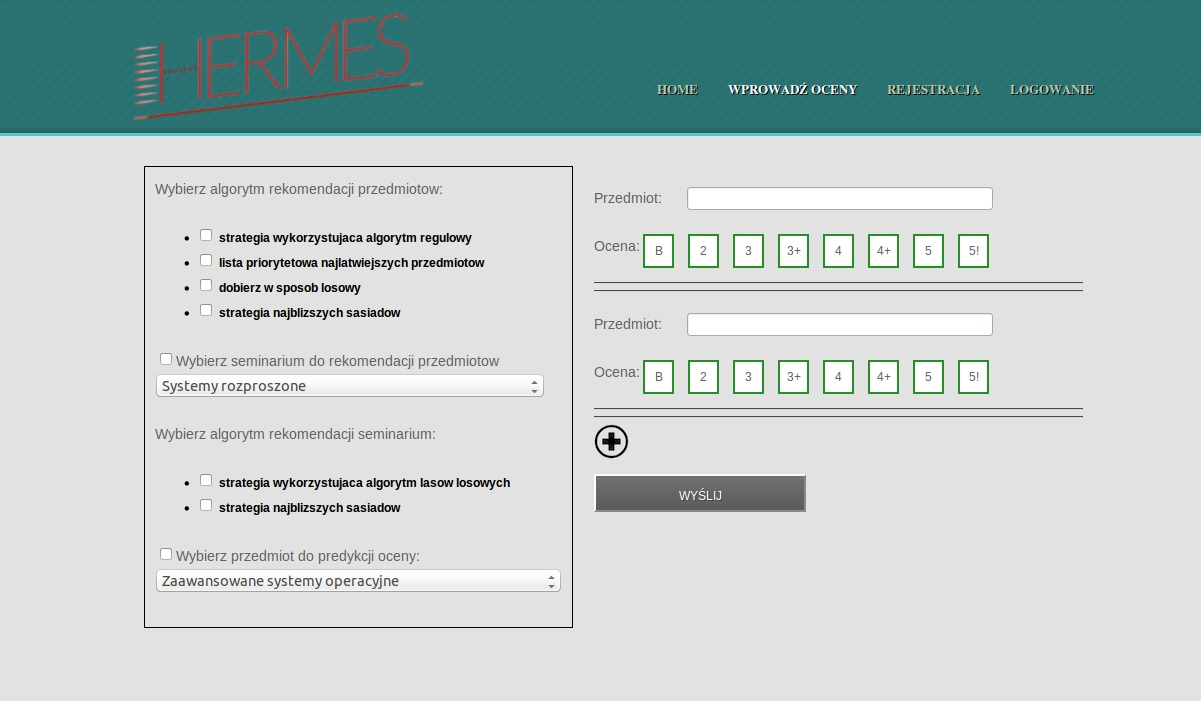
\includegraphics[scale=0.50]{interfejsWstepny.jpg}
	\text{interfejs po wyborze opcji "wprowadź oceny"}
\end{minipage} \\ 

\newpage

\subsubsection{Predykcja ocen}
~\\ \indent
Użytkownik wybiera predykcję oceny z przedmiotu za pomocą opcji "wybierz przedmiot do predykcji oceny" \par
~\\
\begin{minipage}{\linewidth}
	\centering
           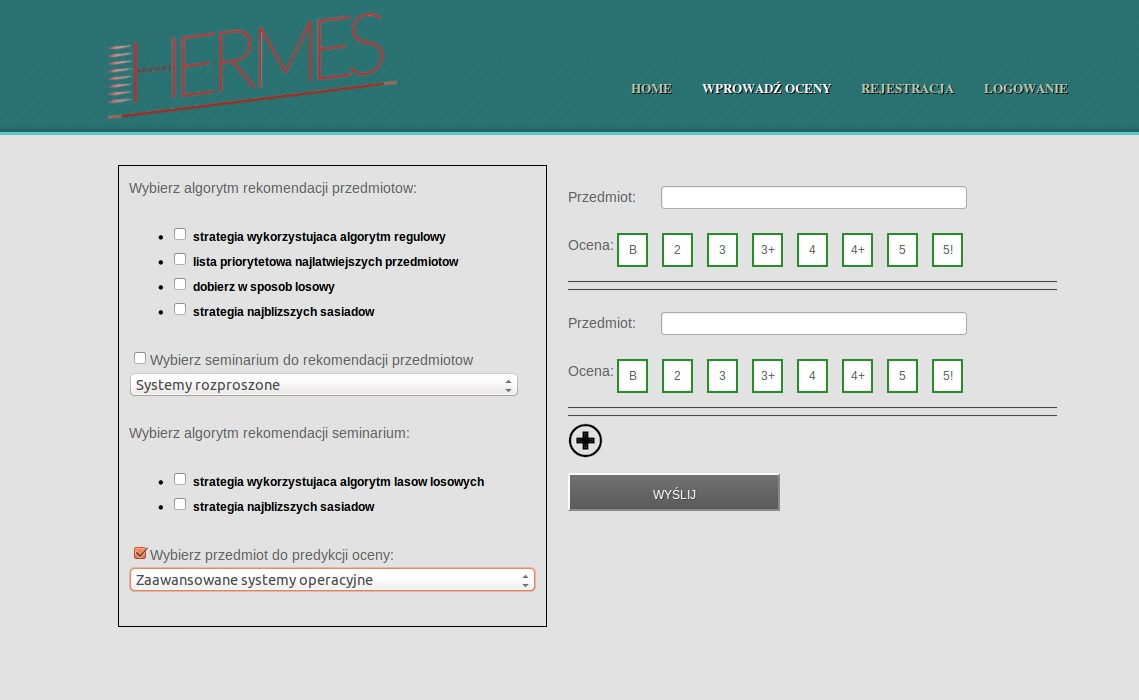
\includegraphics[scale=0.5]{predykcjaPrzedmSelect.jpg}
	\text{wybór opcji predykcji oceny z przedmiotu}
\end{minipage} \\ \\

\newpage
Po wybraniu tej opcji użytkownik może z rozwijanej listy wybrać przedmiot,z którego chce predykcję. ~\\ \par
\begin{minipage}{\linewidth}
          \centering
           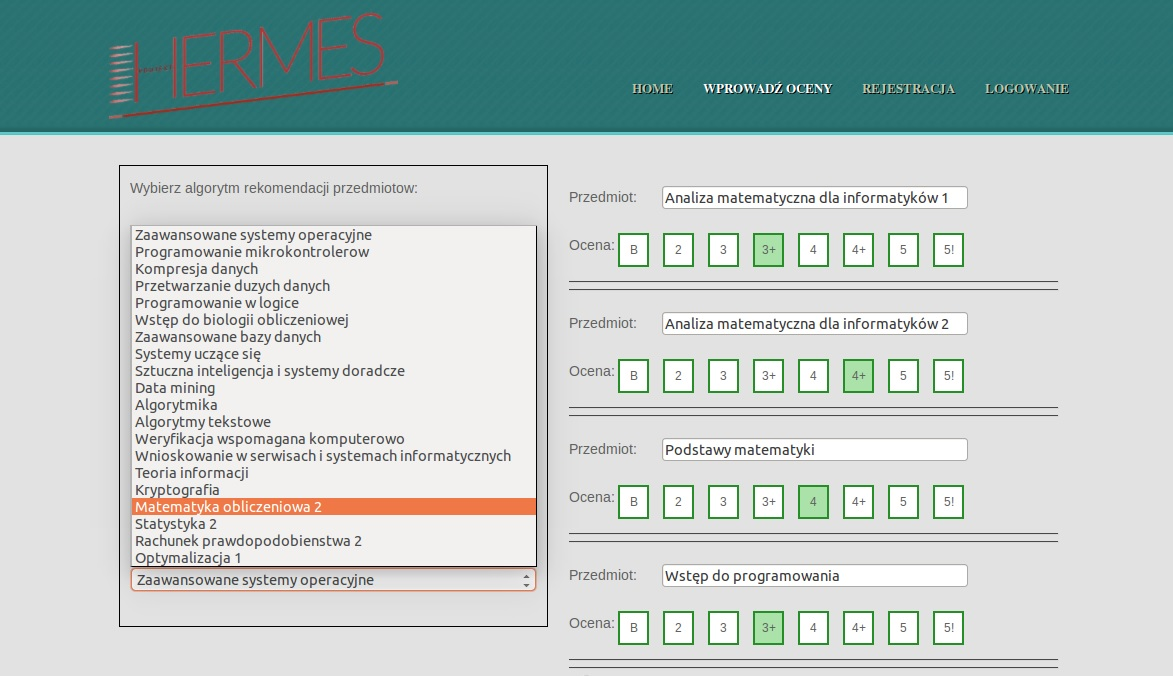
\includegraphics[scale=0.5]{predykcjaPrzedm.jpg}
	\text{wybór przedmiotu do predykcji}
\end{minipage} \\ \\


Po jego wybraniu i użyciu opcji "wyślij"  użytkownik otrzymuje wynik w postaci następującej strony: \\ \par 
 ~\\
\begin{minipage}{\linewidth}
	\centering
           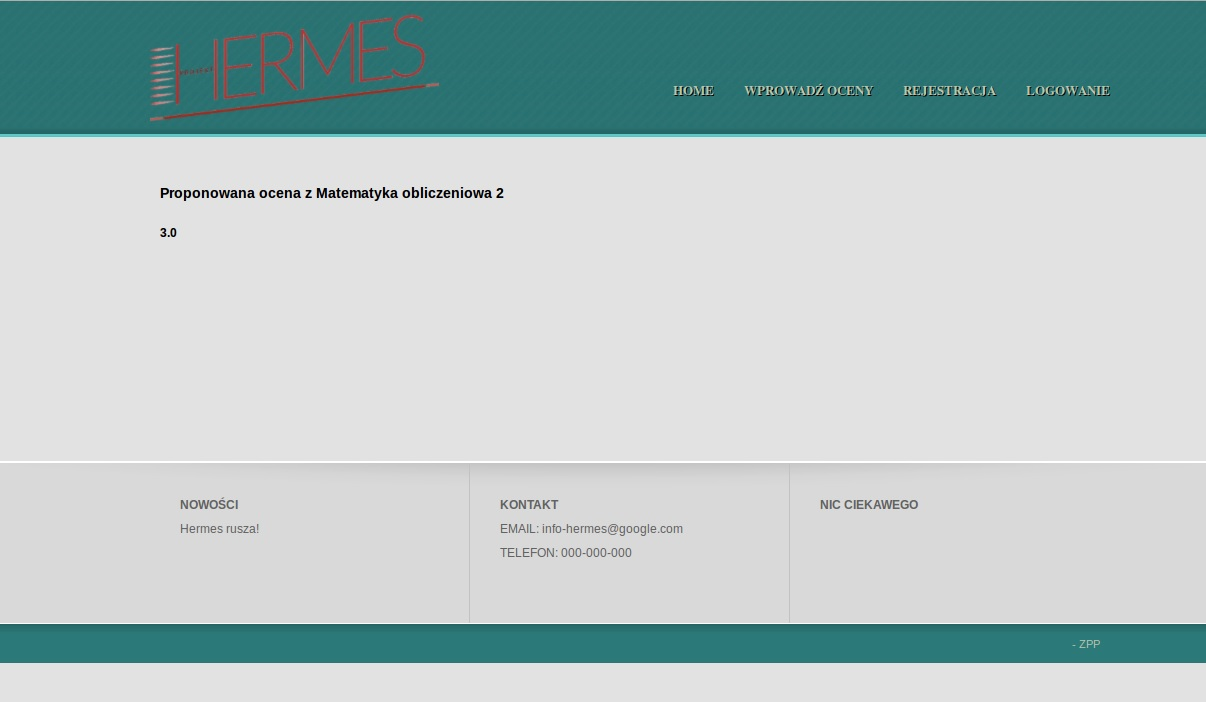
\includegraphics[scale=0.5]{predykcjaPrzedmResult.jpg}
	\text{Przykładowy rezultat zapytania o predykcję oceny}
\end{minipage} \\ 

\subsubsection{Remomendacja seminariów}
~\\ \indent

Użytkownik chcąc otrzymać rekomendowane seminaria musi wybrać opcję otrzymania rekomendacji seminarium wg jednego z dwóch algorytmów: strategii lasów losowych bądź najbliższych sąsiadów. \par 
~\\
\begin{minipage}{\linewidth}
	\centering
           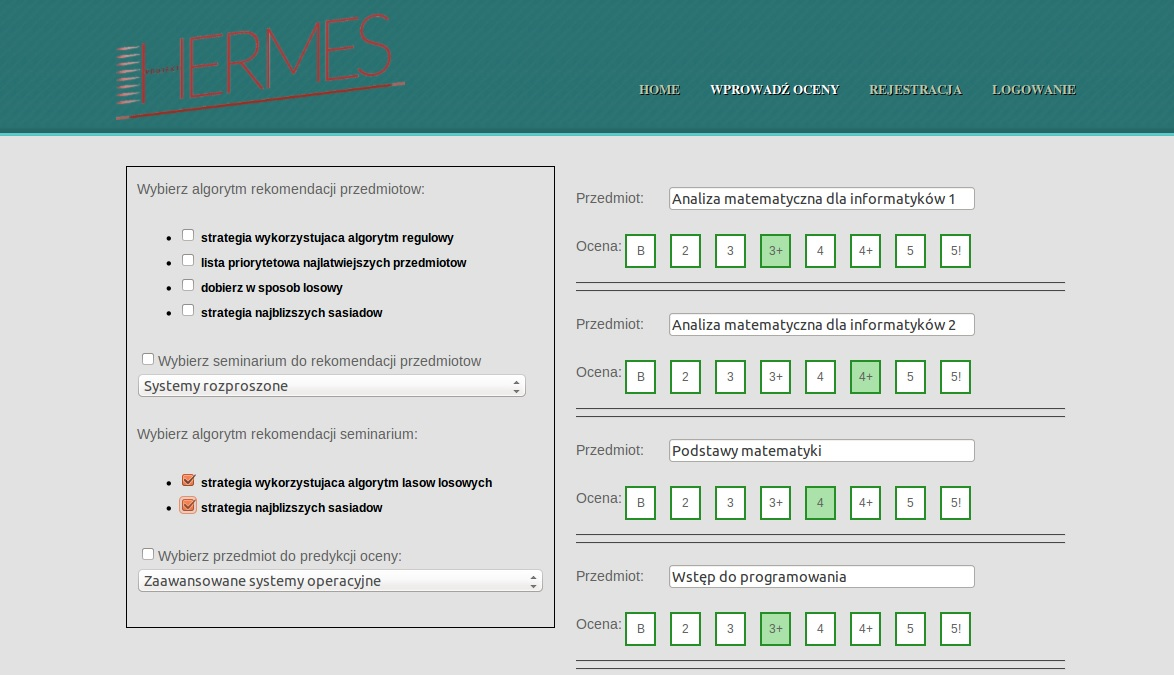
\includegraphics[scale=0.5]{reksem.jpg}
	\text{wybór opcji rekomendacji seminarium}
\end{minipage} \\

\newpage

Na podstawie danych wprowadzonych przez studenta oraz wybranych przez niego algorytmów rekomendacji seminarium student otrzymuje wyniki predykcji \par
~\\
\begin{minipage}{\linewidth}
	\centering
           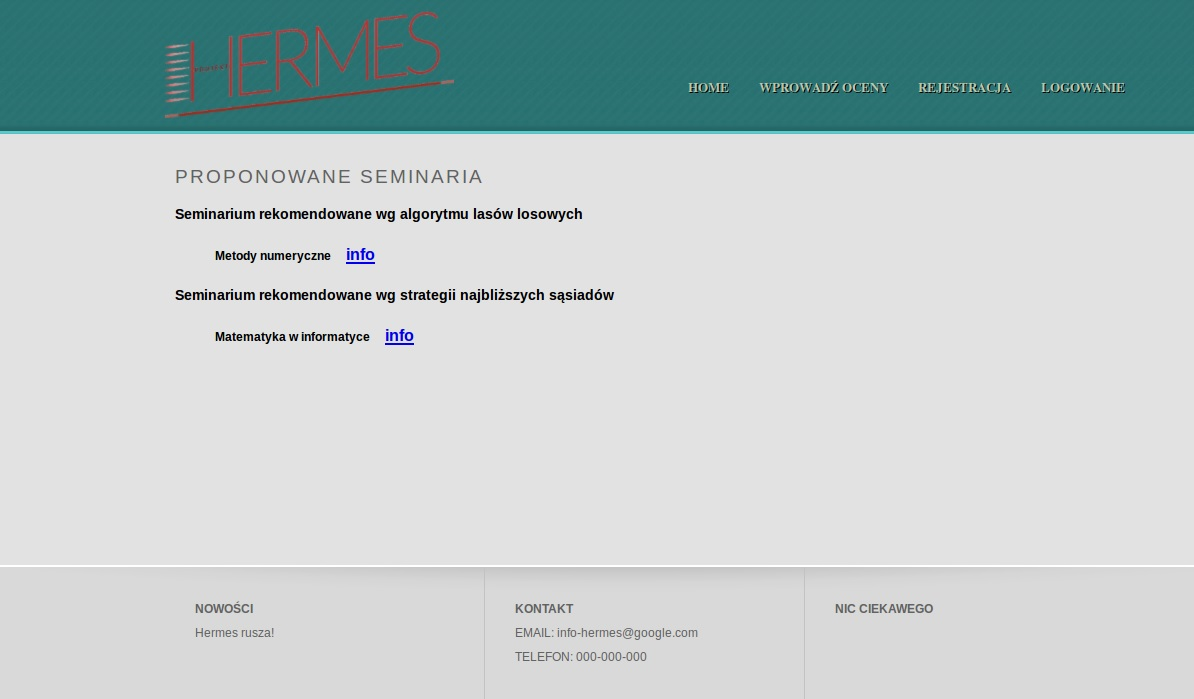
\includegraphics[scale=0.5]{rekSemResult.jpg}
	\text{Przykładowy rezultat prośby o zarekomendowanie seminarium}
\end{minipage} \\  \\ \\
Dla każdego seminarium użytkownik może podejrzeć informacje dotyczące zwróconego przemiotu, takie jak jego strona w systemie usos czy też podstawowe statystyki jak zdawalność i średnia ocena \par
~\\
\begin{minipage}{\linewidth}
	\centering
           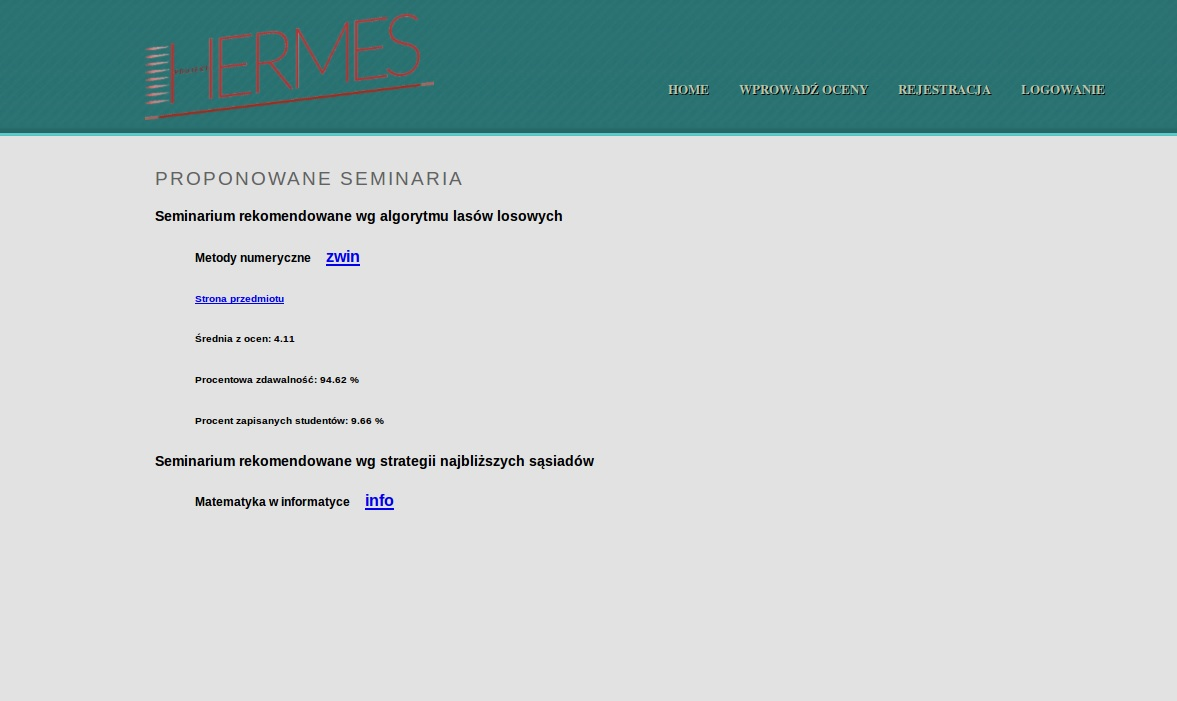
\includegraphics[scale=0.5]{rekSemResultInfo.jpg}
	\text{Przykładowy rezultat prośby o obliczenie rankingu seminariów}
\end{minipage} \\ 


\subsubsection{Rekomendacja przedmiotów} ~\\ \indent
Po wybraniu opcji rekomendacji przedmiotów student otrzymuje wybór kilku opcji. Może wybrać opcje "znajdź najłatwiejsze", szczęśliwy traf - "sposób losowy", "ranking wg algorytmu najbliższych sąsiadów" oraz "znajdź wg algorytmu regułowego". \par
 ~\\
\begin{minipage}{\linewidth}
	\centering
           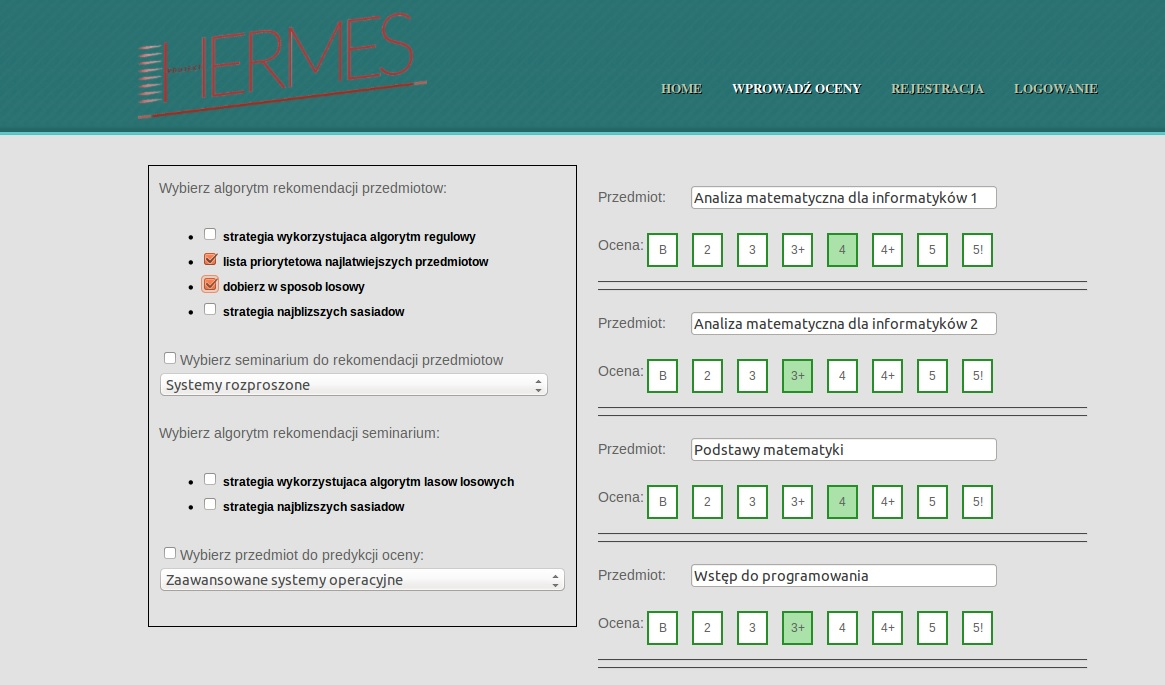
\includegraphics[scale=0.5]{rekPrzedm.jpg}
	\text{Interfejs użytkownika dla opcji rekomendacji przedmiotów - wybór algorytmów}
\end{minipage} \\  \\ \\

\newpage

Jako wynik każdej z tych rekomendacji student otrzymuje ranking 5 przedmiotów które wg danego algorytmu mają największą szansę pasować do zainteresowań studenta. \par
 ~\\
\begin{minipage}{\linewidth} 
	\centering
           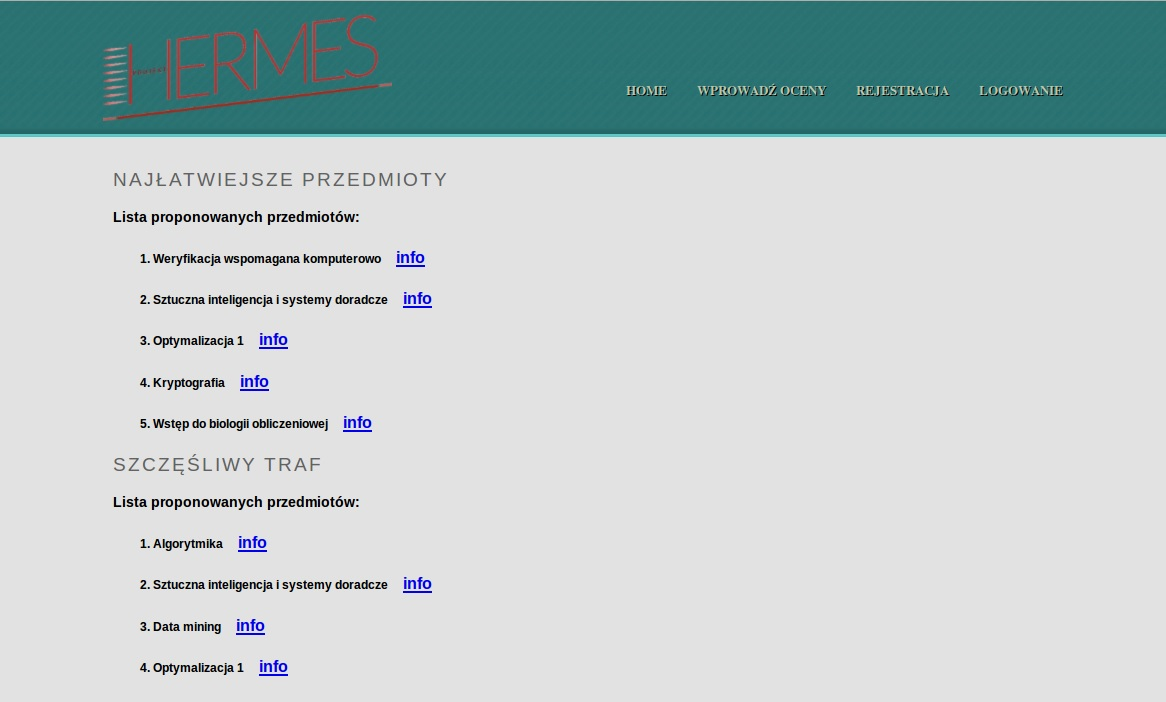
\includegraphics[scale=0.5]{rekPrzedmRank.jpg}
	\text{Przykładowy rezultat dla rekomendacji przedmiotów wg zainteresowań studenta}
\end{minipage} \\ 

Każdy przedmiot po rozwinięciu opisu zawiera proste statystyki, tak jak dla rekomendacji seminariów : ogólną zdawalność, średnią z ocen, ogólny procent studentów uczęszczających na ten przedmiot czy link do strony przedmiotu w systemie USOS. \par
 ~\\
\begin{minipage}{\linewidth}
	\centering
           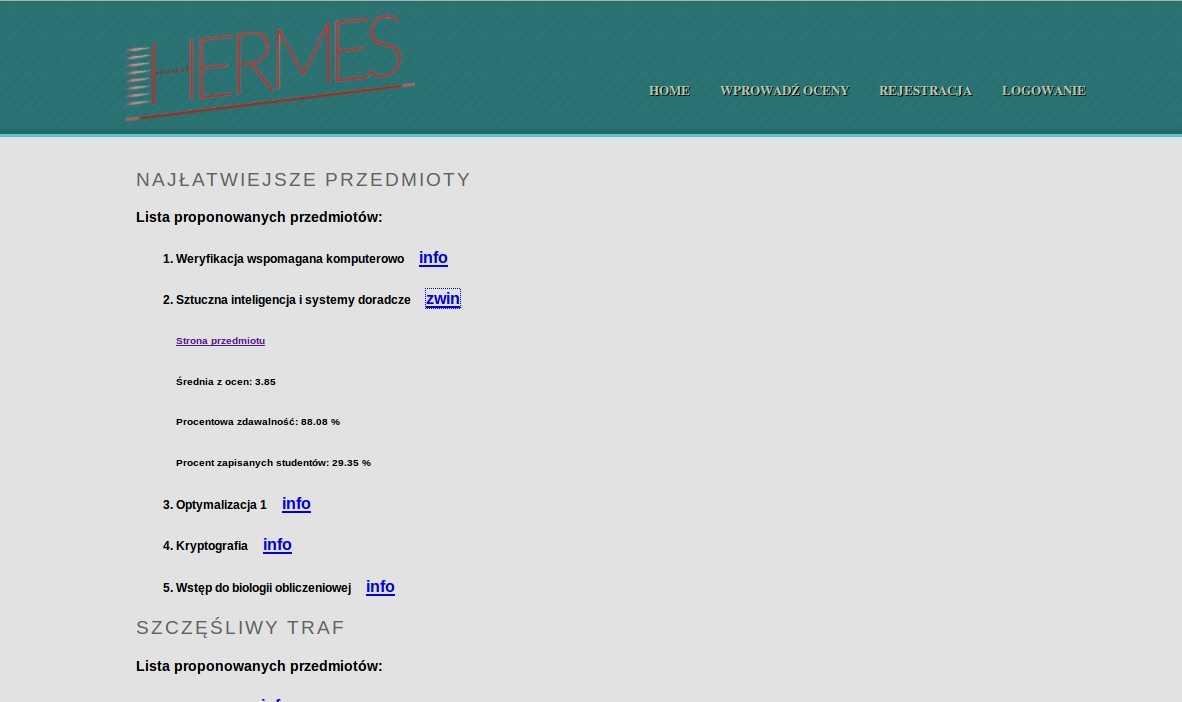
\includegraphics[scale=0.5]{rekPrzedmRankDetails.jpg}
	\text{Opis przedmiotu po rozwinięciu (tu Sztuczna Inteligencja)}
\end{minipage} \\ 

\subsubsection{Rekomendacja przedmiotów do seminarium}

Ostatnią funkcjonalnością dla studenta jest możliwość otrzymania rekomendacji do semianarium. Student, chcąc otrzymać taką predykcje, musi zaznaczyć opcję "Wybierz seminarium do rekomendacji przedmiotów" \par
~\\
\begin{minipage}{\linewidth}
	\centering
           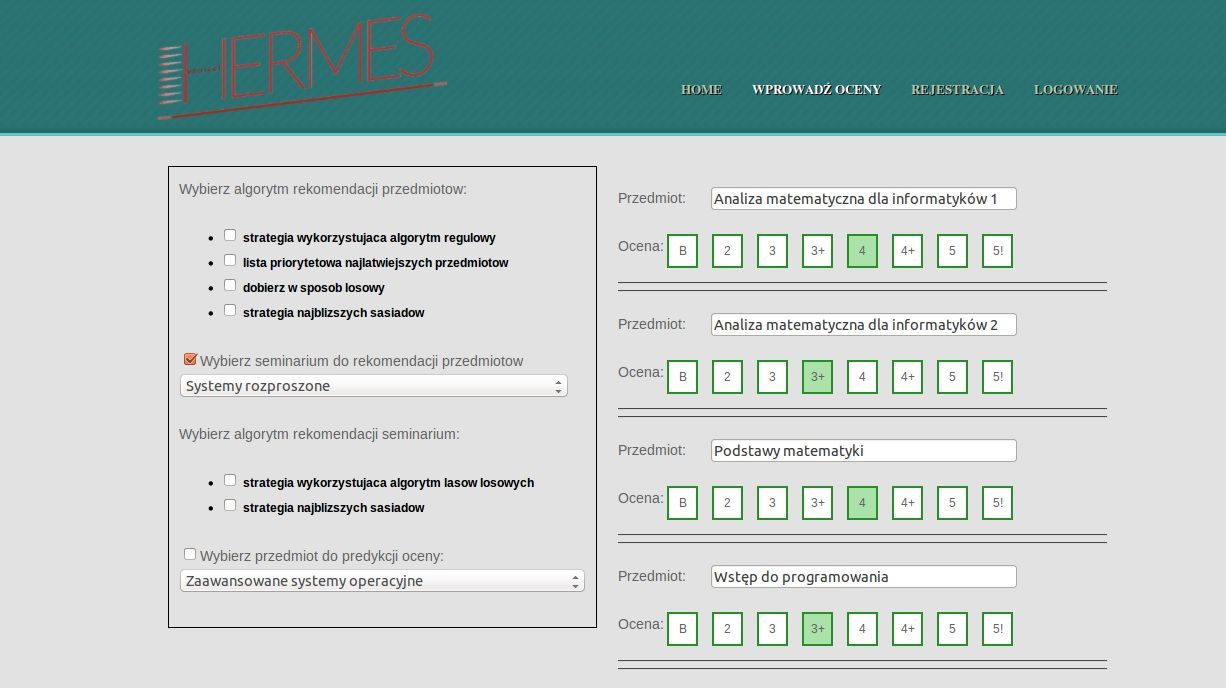
\includegraphics[scale=0.5]{rekPrzedmSem.jpg}
	\text{wybór opcji rekomendacji przedmiotow do seminarium}
\end{minipage} \\ \\
\newpage
Po wybraniu tej opcji student z rozwijanej listy wybiera interesujące go seminarium spośród seminariów znajdujących się w bazie \par
~\\
\begin{minipage}{\linewidth}
	\centering
           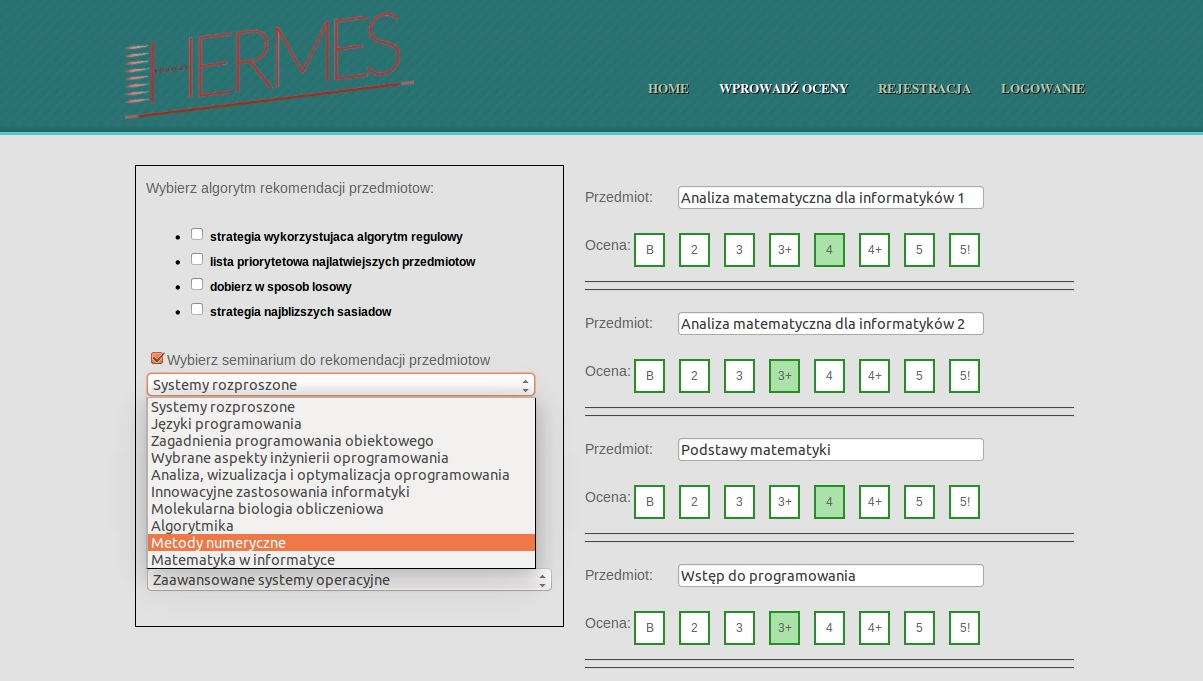
\includegraphics[scale=0.5]{rekPrzedmSemSelect.jpg}
	\text{wybór seminarium do rekomendacji przedmiotów}
\end{minipage} \\ \\

Po użyciu przycisku "wyślij" student otrzymuje ranking 5 najbardziej zgodnych do jego osiągnięć i wybranego seminarium przedmiotów \par
~\\
\begin{minipage}{\linewidth}
	\centering
           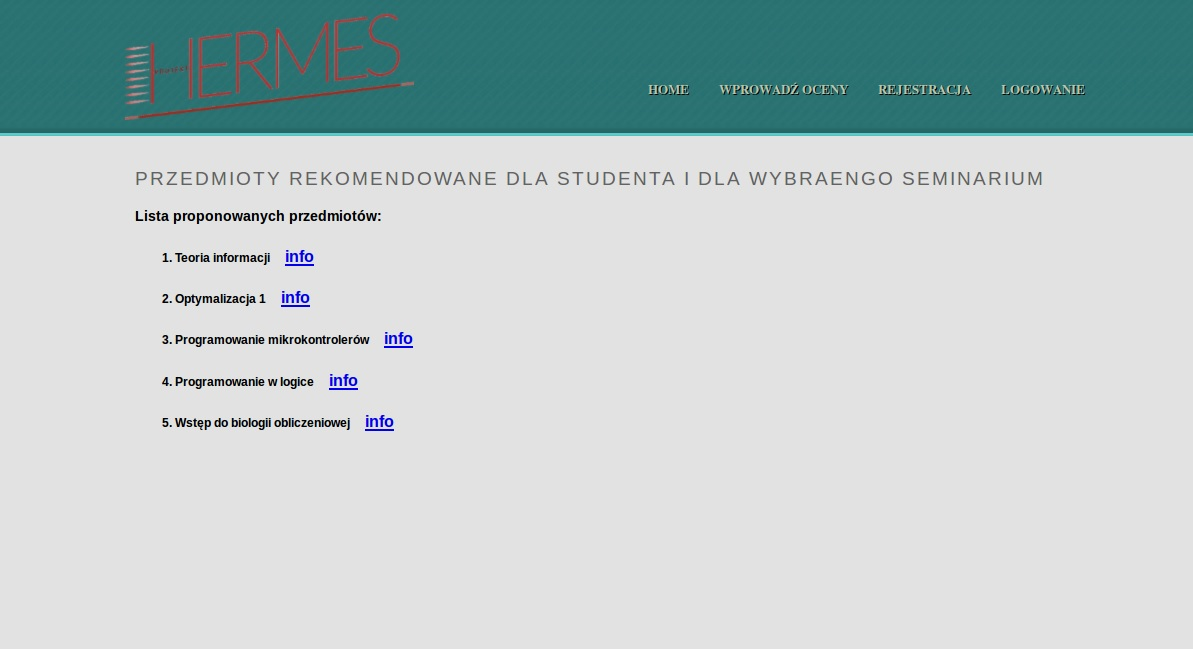
\includegraphics[scale=0.5]{rekPrzedmSemResult.jpg}
	\text{rezultat predykcji przedmiotów związanych z seminarium}
\end{minipage} \\ ~\\
\newpage
Analogicznie do poprzednich funkcjonalności możliwe jest podejrzenie informacji o przedmiotach.

\subsection{Użytkownik zalogowany}

\section{Funkcjonalności dla Administracji}
~\\ \indent
Domyślnie miała być jeszcze funkcjonalność dla administracji, tzn predykcja popularności przedmiotów, niestety zabrakło nam czasu by ją zaimplementować.
 

 \chapter{Architektura} 
\section{Schemat Architektury}
~\\
\begin{minipage}{\linewidth} 
	\centering
           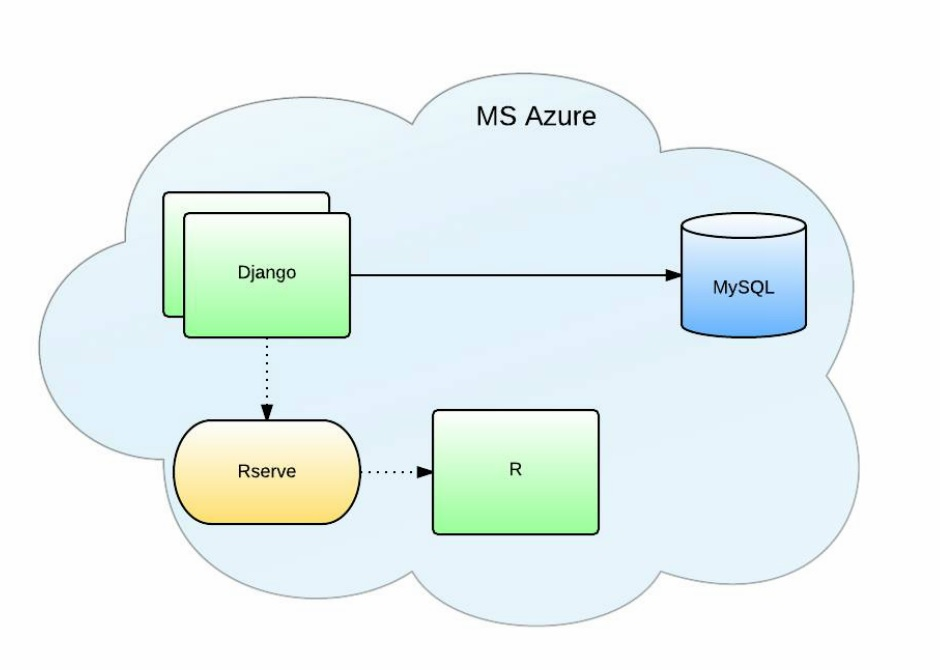
\includegraphics[scale = 0.5]{architekturaFin.jpg}
	\text{Architektura systemu Hermes}
\end{minipage} \\ \\ \\
 W architekturze i logice naszego systemu wyróżniamy następujące komponenty:
 \begin{itemize}
 
\item \textbf{Chmura (MS Azure)} - Sercem systemu jest główny serwer wraz z innymi usługami znajdujący się w chmurze internetowej. Znajduje się na niej serwer bazy danych, serwer WWW oraz serwer usług analitycznych.

\item \textbf {RDB (MySQL)} - Relacyjna baza danych zawierająca statystyczne dane dotyczące zdawalności przedmiotów przez studentów, ich zapełnienia, popularność itd. Stanowi bazę do tworzenia predykcji.

\item \textbf{Sysytem R (R)} - język i zestaw bibliotek uczenia maszynowego wykorzystywany w predykcjach.

\item \textbf{Rserve (Rserve)} - serwer pośredniczący między stroną WWW a systemem R. Strona komunikuje się z R
poprzez komunikaty wysyłane do Rserve.
 

\item \textbf{Strona WWW (Django)} - interfejs za pomocą którego użytkownik może przesyłać prośby o wykonanie udostępnianych przez system rekomendacji.

\item \textbf{Serwer WWW (Django)} - udostępnia użytkownikom stronę internetową, w naszym systemie pośredniczy między interfejsem użytkownika a bazą danych. Pośredniczy również w komunikacji z serwerem analitycznym.

  
\end{itemize}

\section{Schemat współdziałania komponentów architektury i przepływu danych}
~\\
\begin{minipage}{\linewidth} 
	\centering
           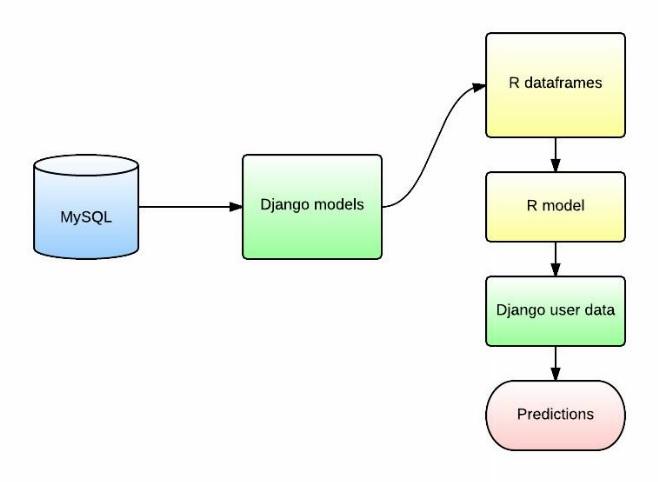
\includegraphics[scale = 0.7]{dataFlow.jpg}
	\text{Schemat przepływu danych w systemie}
\end{minipage} \\ \\ 
~\\ \indent

Schemat działania i komunikacji między poszczególnymi komponentami wygląda następująco:
\begin{enumerate}

\item Na samym początku przy uruchomieniu systemu django ładuje modele na podstawie bazy danych MySQL.

\item R zaczyna przetwarzać dane w bazie i na ich podstawie tworzy dataframes (tzn format danych zgodny z R) które są bazą obliczania predykcji oraz rekomendacji.

\item Po wykonaniu przetworzenia danych i obliczenia statystyk aktywuje się serwer WWW i system staje się dostępny dla użytkowników.

\item Użytkownik wchodzi na stronę i za pośrednictwem jej interfejsu może przesłać do serwera prośbę o rekomendację bądź predykcję.

\item Serwer WWW po odebraniu prośby o rekomendacje przesyła żądanie do Rserve z poleceniem obliczenia predykcji, wykorzystując się przy tym odebrane wcześniej dane użytkownika.

\item R dokonuje obliczeń na podstawie wyliczonego wcześniej modelu i zwraca do serwera WWW predykcję jako model R.

\item Serwer WWW odbiera rezultat zapytania, konwertuje go na format zgodny z formatem Django i wyświetla go użytkownikowi za pośrednictwem strony WWW.

\end{enumerate}


 \chapter{Technologia}
Technologie wykorzystywane w naszym systemie: \par

 \begin{minipage}{\linewidth}
            \centering
            
\includegraphics[width=10cm, height = 3cm]{azure.jpg}
\end{minipage} \\ \\
\noindent 
 \textbf{Microsoft Azure} - Azure jest komercyjną platformą obsługiwaną przez Microsoft. Udostępnia ona usługi związane z chmurą internetową (tzw cloud-computing). W naszym systemie znajduje sie na niej serwer WWW a także serwer bazy danych. \par ~\\
\begin{minipage}{\linewidth}
            \centering
            
\includegraphics[width=8cm, height = 3cm]{mysql.png}
\end{minipage} \\ \\

\noindent \textbf{MySQL} - Jeden z najpopularniejszych serwerów relacyjncyh baz danych. Znajduje się w nim relacyjna baza danych zawierająca dane niezbędne do stworzenia modeli uczenia maszynowego.  \par ~\\

\begin{minipage}{\linewidth}
            \centering
            
\includegraphics[width=4cm, height = 4cm]{R.png}
\end{minipage} \\ \\

\textbf{R} - język i zestaw bibliotek używany w celu analizy danych a także obliczania predykcji dla studentów bądź uniwersytetu. \par
\begin{itemize}

\begin{figure}
\centering
\begin{minipage}{0.45\textwidth}
\centering

\includegraphics[width=6cm, height = 3cm]{python-logo-master-v3-TM.png}
\end{minipage}\hfill
\begin{minipage}{0.45\textwidth}
\centering

\includegraphics[width=6cm, height = 3cm]{django-logo-negative.png}
\end{minipage}
\end{figure}

\item \textbf{Python oraz Django} - technologie, za pomocą których tworzymy webowy interfejs użytkownika. \par ~\\

\begin{minipage}{\linewidth}
            \centering
            
\includegraphics[width=7cm, height = 2.5cm]{usosapi.jpg}
\end{minipage} \\ \\

\item \textbf {USOS Api} - API udostępniane przez system USOS. Nasz system wykorzystuje go w celu zebrania danych zalogowanego użytkownika
niezbędnych do rekomendacji.

\end{itemize}

\chapter{Zastosowane Algorytmy}
~\\ \indent Przy tworzeniu algorytmów wykorzystaliśmy pakiet statystyczny R. Gwarantował on dużą kontrolę nad algorytmami,
których używaliśmy. W naszej pracy pojawlły się wszystkie najważniejsze rodzaje algorytmów używanych w eksploracji danych:
\begin{itemize}
 \item klasyfikacja
 \item poszukiwanie reguł asocjacyjnych
 \item grupowanie
\end{itemize}
Najwięcej pojawiło się zastosowań pierwszej z metod. Czasem używaliśmy też podejścia statystycznego, nie ucząc jakiegoś modelu,
lecz podejmując decyzje na podstawie statystyk. W zastosowanych algorytmach często używalismy odpowiednio zdefiniowanej
funkcji odleglości między obiektami w naszym modelu. Obiektem był tu wektor $n$-elementowy ocen studenta pomnożonych o 2 oraz 11
w przypadku oceny $5!$ a także $0$, gdy student nie uczestniczył w przedmiocie, dla dwóch takich wektorów definiujemy miarę 
odleglości między studentami $v=(v_{1},..,v_{n})$ i $w=(w_{1},..,w_{n})$:
\[
 dist(v,w) = \sum_{k=1}^n \begin{cases} 10 &\text{gdy } (v_{k} = 0)\oplus(w_{k} = 0) \\|w_{k}-v_{k}| &\text{wpp}  \end{cases}
\]
kod w R:
\lstinputlisting{dist.R}
Podana funkcja mocniej wyraża fakt, że studenci brali różne przedmioty niż to że mieli różne oceny. Uzywaliśmy
jej w algorytmach opartych na metodzie k najbliższych sąsiadow, której używalismy w wielu predykcjach. W naszym systemie 
mieliśmy kilka rodzajów predykcji i rekomendacji:
\begin{itemize}
 \item proponowanie przedmiotów
 \item predykcja seminarium
 \item predykcja ocen
\end{itemize}
\subsection{Algorytmy użyte przy proponowaniu przedmiotów}
Przy proponowaniu przedmiotów obieralnych użylismy 4 strategie:
\begin{itemize}
 \item wyliczanie reguł asocjacyjnych
 \item strategia najbliższych sąsiadów
 \item przydział w oparciu o statystyki
 \item przydział losowy
\end{itemize}
Reguły asocjacyjne wyliczyliśmy za pomocą algorytmu apriori dostępnego w pakiecie 'arules'. Algorytm brał na wejściu koszyki
przedmiotów, czyli zestawy przedmiotów obieralnych, które wzięli poszczególni studenci, zaś na wyjściu zwracał reguły postaci
'jeśli student wziął przedmioty $p_{1},..,p_{k}$ to prawdopodobnie weźmie też przedmiot $p_{l}$'. To 'prawdopodobnie' 
zależy od miar $support$ i $confidence$ podawanych na wejściu algorytmu.
Miary $support$ i $confidence$ ustawiliśmy tak, by reguł nie bylo za duzo, ale też byly sensowne. \\
Strategia najbliższych sąsiadów została użyta w oparciu o miarę $dist$ przedstawioną wyżej. Polegała ona na tym, że 
spośród pewnej liczby najbliższych studentowi, któremu chcemy coś zaproponować, sasiadów, bierzemy przedmioty, które oni brali.
W tym podejściu próbujemy zaklasyfikować studenta do podobnej grupy i przydzielić mu to co brali 'podobni' studenci. Kod w R:
\lstinputlisting{nearestSub.R}
Przydział w oparciu o statystyki to propozycja przedmiotów, które prawdopodobnie byłoby studentowi najłatwiej zaliczyć.
Statystykę 'łatwości' przedmiotu stanowiła średnia ważona supportu, średniej ocen i zdawalności przedmiotu. \\
Przydział losowy polegał na braniu z jenostajnym rozkładem prawdopodobieństwa przedmiotów, których student jeszcze nie wziął.
\subsection{Algorytmy używane przy predykcji seminariów}
Przy proponowaniu seminariów użylismy 2 strategii:
\begin{itemize}
 \item klasyfikator najbliższych sąsiadów
 \item klasyfikator lasów losowych
\end{itemize}
Klasyfikator najbliższych sąsiadow, tak jak w przypadku proponowania przedmiotów, równiez korzystał ze zdefniowanej funkcji
odleglości i ze zbioru decyzji dla najbliższych sąsiadów, czyli seminarium, które wybrali najbliżsi sąsiedzi, jako proponowane
wybierał mode, czyli najczęściej występujące wśród sąsiadów seminarium. \\
Klasyfikator lasów losowych budowaliśmy w oparciu o pakiet 'randomForest'. Jest to klasyfikator, który buduje sie w oparciu o
klasyfikacje na pewnej liczbie drzew decyzyjnych, następnie agregując decyzje z tych drzew, najczęściej przez głosowanie.
Dawał on gorsze wyniki niz klasyfikator najbliższych sąsiadow.
Na danych testowych,skuteczność klasyfikatora knn wynosiła $0.45$ podczas gdy skuteczność lasów losowych tylko $0.26$. Jednak
zaletą tego klasyfikatora jest to, że buduje on już wcześniej model i decyzja dla danych wejściowych studenta obliczana
jest bardzo szybko, w przeciwieństwie do klasyfikatora knn. Kod w R:
\lstinputlisting{rf.R}
\subsection{Algorytmy używane przy predykcji ocen}
Przy predykcji ocen użyliśmy wyłącznie klasyfikatora najbliższych sąsiadów. W przypadku wyboru algorytmu uczenia nadzorowanego, musielibyśmy trenować nasz klasyfikator dla każdego przedmiotu, co przy dużej 
liczbie przedmiotów jest zadaniem dość karkołomnym. Dlatego zdecydowaliśmy się na algorytm uczenia nienadzorowanego, który dobrze się sprawdzał w poprzednich predykcjach. Tutaj algorytm wybiera 100 najbliższych sasiadów i wybiera tych, którzy wzięli dany przedmiot, następnie przelicza średnią ocen
wybranych studentów z tego przedmiotu i zwraca ją jako wynik klasyfikacji.


\chapter{Organizacja pracy oraz podział obowiązków} ~\\

\section{Praca nad systemem} ~\\

Za namową zamawiającego na początku zdecydowaliśmy się zrealizować projekt za pomocą technologii koncernu Microsoft. Otrzymaliśmy od niego licencję Bizspark która dała nam licencję na swobodne wykorzystywanie produktów Microsoftu przez 2 lata. Dodatkowo Bizspark umożliwiał korzystanie z usługi Azure w zakresie abonamentu w wysokości 150 euro na miesiąc. Dlatego wybraliśmy chmurę Azure jako nasz serwer. Planowaliśmy dodatkowo zrealizować obliczanie predykcji za pomocą Sql Server Analysis Services a frontend za pomocą .NET. \\

Z projektem jednak wiązały się dość znaczące problemy. Pierwszym z nich była zmiana technologii użytej w celu obliczania predykcji, na którą zdecydowaliśmy się w lutym. Przed rozpoczęciem pracy nad projektem nikt z nas nie znał możliwości Sql Server Analysis Services (SSAS) ani nie tworzył strony internetowej w .NET. O ile z .NET nie było znaczących problemów, usługi analityczne Sql Servera stanowiły dla nas barierę nie do przejścia. Ze względu na dość kiepsko udomkumentowną technologię SSAS, brak obiecanych szkoleń z tej technologii oraz brak zajęć na uniwersytecie jej poświęconym a także małej elastyczności algorytmów tej usługi podjęliśmy decyzję o rezygnacji z tego narzędzia. Zdecydowaliśmy się na wykorzystanie języka skryptowego R, z którym dobrze zaznajomione były 2 osoby w zespole. Zmieniliśmy także realizację frontendu z .NET na Django ponieważ główny powód wyboru .NET - pluginy dedykowane dla SSAS, przestał być ważny dla projektu. Z Django obeznane były wszystkie osoby w zespole, a dodatkowym atutem tego wyboru był jeden członek zaspołu posiadającz doświadczenie zawodowe w pisaniu aplikacji w Pythonie. \\

Kolejnym znaczącym problemem przy realizacji projektu była mocno utrudniona praca związana z analizą danych i dobieraniem optymalnych algorytmów. Zamawiający obiecał nam dostarczenie zaszumionych danych z systemu USOS. Czekaliśmy na nie, ponieważ trudno było samemu wymyślić i wygenerować nietrywialne korelacje, zbliżone do rzeczywistości. Próbka takich danych mocno pomogłaby nam z doborem algorytmów predykcyjnych. Jednak zaszumienie okazało się w praktyce niemożliwe a "zwykłych" danych nie mogliśmy otrzymać z powodu ustawy o ochronie danych osobowych. O tych ograniczeniach praktycznie dowiedzieliśmy się dopiero w kwietniu, co mocno nam popsuło pracę nad algorytmami predykcyjnymi i analizą ich jakości która niestety nie została wykonana na danych produkcyjnych.

\section{Organizacja Pracy} ~\\


W naszej pracy korzystaliśmy z repozytorium git. Było ono umieszczone na stronie \\ \textit{http://www.github.com}. W ramach tego repozytorium mieliśmy następujące odnogi:
\begin{itemize}
    \item \textbf{ZPP-frontend} - pierwsza wersja frontendu, zrealizowana w technologii C\# .NET, a w kolejnej iteracji za pomocą pluginu do django w Visual Studio 2013
    \item \textbf{ZPP-Frontend2.0} - druga odnoga reprezentująca frontend realizowany w django na systemie linux. Jest to odnoga w której został stworzony końcowy efekt naszej pracy.
    \item \textbf{ZPP-SSDT} - nazwa tej odnogi bierze się od Sql Server Data Tools - na początku trzymaliśmy w tym repozytorium projekty Sql Server Analysis Services zajmujące się analizą danych. W kolejnej iteracji w tym repozytorium umieszczane były skrypty obliczające rekomendacje w języku R.
    \item \textbf{ZPP-slides} - w tej odnodze tworzona i przechowywana była prezentacja końcowa.
    \item \textbf{ZPP-pracalic} - odnoga w której powstawała praca licencjacka.
\end{itemize} ~\\

Przydział zadań do osób i planowanie pracy zostały zrealizowane za pomocą portalu Redmine. \\

Praca na początku projektu przebiegała dość chaotycznie, z długimi przerwami. Dużą blokadą były dla nas problem z efektywną pracą nad predykcjami z SSAS oraz brak danych bliższych rzeczywistości utrudniający nam wyjście poza teoretyczne rozważanie o algorytmach. Jednak pewne prace były wzwiązku z tym systemem wykonywane, zbudowaliśmy pewną strukturę danych, wygenerowaliśmy dane testowe i próbowaliśmy generowac predykcję. Z wszystkich tych rzeczy (nie licząc części danych testowych) zrezygnowaliśmy w dalszej fazie realizacji projektu.

Realną pracę wychodzącą poza studiowanie dokumentacji i metodę prób i błędów prowadząca do nikąd zaczęliśmy dopiero po decyzji o zmianie technologii w lutym. Praca odbywała się wtedy w cotygodniowych iteracjach, a znacząco przyśpieszyła w kwietniu po ostatecznej decyzji o braku możliwości otrzymania jakichkolwiek danych przypominających rzeczywiste. Niestety ze względu na niezbyt długi pozostały wówczas czas nie udało nam się zrealizować wszystkich funkcjonalności, w szczególności integracji z USOS (przez brak czasu ale także utrudnioną współpracę z zamawiającym).

\section{Podział Obowiązków} ~\\

TODO (przy działającym serwisie rzetelnie opiszę wkład osób)
~\\ \indent W projekcie Hermes podział pracy był następujący:

\begin{itemize}
\item \textbf{Tomasz Grabowski} :
    \begin{itemize} 
    \item Pisanie licencjatu : jego redakcja, formatowanie, wstawienie zrzutów ekranu. Napisanie wszystkich rozdziałów poza rozdziałem 5 (autorstwa Krzystofa Rutkowskiego) oraz tym podrozdziałem (każdy sam opisywał swój wkład).
    \item Pomoc przy tworzeniu frontendu, w szczególności: edycja szablonu wyświetlającego wyniki predykcji oraz rekomendacji, obliczanie i wyświetlanie statystyk każdego przemiotu (po uzyciu w tym szablonie opcji info), realizacja tego elementu w Django (kod w języku Python). 
    \item Generowanie danych testowych i przypadków testowych .
    \item Funkcjonalne testowanie systemu. 
    \item We wstępnej wersji projektu (gdy jeszcze korzystaliśmy z Sql Server Analysis Services) tworzenie przypadków oraz danych testowych a także projektowanie kostki OLAP i sposobu wykorzystania modułu Data Mining w celu obliczenia rekomendacji.
    \end{itemize}

\item \textbf{Adam Markiewicz}:
	\begin{itemize}
	        \item Tworzenie frontendu - modele ORM, szablony, obsługa logowania, rejestracji i edycji ocen użytkowników, zintegrowanie bazy ocen użytkowników z resztą frontendu (kod w Pythonie i Javascripcie), debugowanie
	        \item Administrowanie serwerem WWW i bazą danych, wdrożenie systemu.
	        \item Testy funkcjonalne systemu.
	        \item We wstępnej wersji projektu korzystającej z SSAS - administracja serwerem WWW, hurtownią danych i kontrolerem domeny; projektowanie kostki OLAP i integracja jej z warstwą Data Mining w SSAS.
	    \end{itemize}
\item \textbf{Albert Rozmus} - Pomoc przy tworzeniu frontendu i serwera WWW, prezentacja.
\item \textbf{Krzysztof Rutkowski} :
    \begin{itemize}
        \item organizacja oraz zarządzanie pracą zespołu.
        \item znalezienie osoby która podjęła się stworzenia plakatu.
        \item tworzenie, implementacja i testowanie algorytmow uczenia maszynowego w R.
        \item integracja skryptow R z frontendem.
        \item pomoc przy tworzeniu frontendu: formularze do predykcji ocen i przedmiotów z seminarium, stworzenie modulu dla skryptów R, poprawianie jego błędów
    \end{itemize}
\item \textbf{Wiktor Zuba} - Tworzenie danych testowych do bazy oraz ich relacyjnego modelu. 
\end{itemize}

Plakat został zrealizowany przez osobę wynajętą przez nas w tym celu.

\chapter{Podsumowanie} ~\\ \indent


Projekt napotkał na duże przeszkody w trakcie realizacji. Problemy z zamawiającym, z otrzymaniem sensownych danych testowych oraz z nauką Sql Server Analysis Services a także skutecznym wykorzystaniem jego algorytmów z dość znaczącymi limitacjami mocno wpłynęły na czas spędzony na efektywnej pracy nad projektem. Z ubolewaniem przyznajemy, iż realną pracę przynoszącą progres a nie błądzenie w ślepych zaułkach, książkach i dokumentacjach zaczęliśmy dopiero w marcu.

W celu realizacji projektu i usprawnienia pracy musieliśmy podjąć decyzję o zmianie technologii. Umożliwiło nam to mieć większy wpływ na tworzone algorytmy predykcyjne oraz sposób ich działania. Dużym plusem tej zmiany była możliwośc wykorzystania solidnej znajomośc teorii systemów decyzyjnych oraz jej zastosowania w R przez członków zespołu. Zmiana na Django także była skutkiem lepszej znajomości Pythona przez zespół. Uważamy, iż zmiany okazały się w końcowym rozrachunku pozytywne, ponieważ udało nam się zaimplementować system który zawiera większość planowanych na początku funkcjonalności. Dodatkowo, dzięki zastosowanym technologiom, w miarę łatwe jest rozwijanie systemu. W celu zaimplementowania nowych typów predykcji wystarczy napisać nowy skrypt w R i załączyć go do systemu oraz zintegrować z frontendem.

Problemy przy pracy nad projektem niestety uniemożliwiły spełnienie naszych wszystkich założeń. Zabrakło nam czasu na zaimplementowanie funkcjonalności dla pracowników predykujących popularność wybranych przedmiotów wśród studentow. Z przyczyn niezależnych od nas nie udało nam się również przetestować napisanych przez nas algorytmów na prawdziwych danych, przez co nie mieliśmy możliwości praktycznej weryfikacji predykcji. 

Mamy jednak nadzieję, iż pomimo tych trudności system sprawdzi się na prawdziwych danych i okaże się realną, efektywną pomocą dla studentów.


\begin{thebibliography}{99}
\addcontentsline{toc}{chapter}{Bibliografia}
\bibitem[AZR]{AZR} Microsoft
\textit{dokumentacja techniczna Azure} \\
http://azure.microsoft.com/en-us/documentation/
\bibitem[PTN]{ptn}
Python Software Foundation
\textit{dokumentacja techniczna języka Python} \\
https://docs.python.org/2.7/
\bibitem[DGO]{DGO} Django Software Foundation
\textit{dokumentacja techniczna Django} \\ 
https://docs.djangoproject.com/en/1.8/
\bibitem[R]{R} R Development Core Team
\textit{dokumentacja techniczna języka R} \\
http://cran.r-project.org/manuals.html
\bibitem[RSV]{RSV} Simon Urbanek
\textit{dokumentacja techniczna serwera R - modułu RServe} \\
http://www.rforge.net/Rserve/doc.html
\end{thebibliography}


\end{document}